\chapter{Evaluation}
\section{Bewertungskriterien}
\subsection{Diskriminator-Verlust}
Der Diskriminator-Verlust ist ein wesentliches Maß für die Effektivität des Diskriminators in einem GAN-Modell. Ein niedriger Diskriminator-Verlust bedeutet, dass der Diskriminator erfolgreich zwischen echten und generierten Bildern unterscheiden kann. Im Kontext eines GANs zeigt ein abnehmender Diskriminator-Verlust über die Epochen hinweg, dass der Diskriminator zunehmend besser darin wird, die Authentizität der Bilder zu beurteilen. Ein hoher Diskriminator-Verlust weist hingegen darauf hin, dass das Modell Schwierigkeiten hat, echte von generierten Bildern zu unterscheiden, was ein Indikator für Verbesserungspotenzial im Training oder der Modellarchitektur sein könnte.

\subsection{Generator-Verlust}
Der Generator-Verlust ist ein Indikator für die Fähigkeit des Generators, Bilder zu erzeugen, die vom Diskriminator als echt eingestuft werden. Ein hoher Generator-Verlust deutet darauf hin, dass der Generator die realen Daten noch nicht effektiv nachahmen kann, während ein niedriger Generator-Verlust ein Zeichen dafür ist, dass die generierten Bilder den echten immer ähnlicher werden. Im Verlauf des Trainings sollte der Generator-Verlust tendenziell abnehmen, was darauf hindeutet, dass der Generator lernt, überzeugendere Bilder zu produzieren.

\subsection{Diskriminator Genauigkeit}
Die Diskriminator-Genauigkeit gibt an, wie oft der Diskriminator korrekt zwischen echten und gefälschten Bildern unterscheidet. Eine hohe Genauigkeit bedeutet, dass der Diskriminator effektiv arbeitet, während eine niedrige Genauigkeit auf Probleme bei der Unterscheidung hinweisen kann. Es ist wichtig, ein Gleichgewicht zu finden, denn eine zu hohe Genauigkeit kann darauf hindeuten, dass der Diskriminator die generierten Bilder zu leicht erkennt, was auf ein Problem mit dem Generator hinweisen könnte.\newline
In einem ideal funktionierenden GAN sollte der Diskriminator eine Genauigkeit von etwa 50$\%$ erreichen. Das bedeutet, dass der Diskriminator die echten von dem generierten Bildern nur zufällig unterscheiden bzw. nicht mehr zuverlässig unterscheiden kann, was zeigt dass das GAN gut trainiert wurde.

\subsection{SSIM-Score (Structural Similarity Index)}
Der SSIM-Score ist ein Maß für die visuelle Ähnlichkeit zwischen den generierten Bildern und den entsprechenden Originalbildern. Er bewertet die Bildqualität anhand von Faktoren wie Helligkeit, Kontrast und Struktur. Ein hoher SSIM-Wert deutet darauf in, dass die generierten Bilder den echten Bildern sehr ähnlich sind, was ein Zeichen für eine hohe Bildqualität ist. Ein niedriger SSIM-Wert kann auf deutliche Unterschiede in der visuellen Struktur hinweisen, was Verbesserungsbedarf im Generator-Training oder in der Modellarchitektur signalisiert.

\section{Pix2Pix: Ergebnisse und objektive Bewertung}
\subsubsection{Evaluierung der Trainingsresultate nach 100 Epochen}
Die Evaluierung der Trainingsresultate des Pix2Pix-Modells basiert auf einer Analyse der 100 durchgeführten Trainingsepochen. Während dieser Epochen wurden spezifische Metriken wie Generator- und Diskriminator-Verluste sowie Diskriminator-Genauigkeit und der Structural Similarity Index Measure (SSIM) überwacht. \newline
Der Generatorverlust zeigte eine anfängliche Tendenz zur Reduktion von 13.782 auf 10.581, was auf eine erfolgreiche Anpassung des Modells an die Trainingsdaten hindeutet. Parallel dazu reduzierte sich der Diskriminatorverlust von 1.009 auf 0.323, was auf eine effiziente Differenzierung zwischen realen und generierten Bildern durch den Diskriminator hinweist.
\begin{figure}[h]
	\centering
	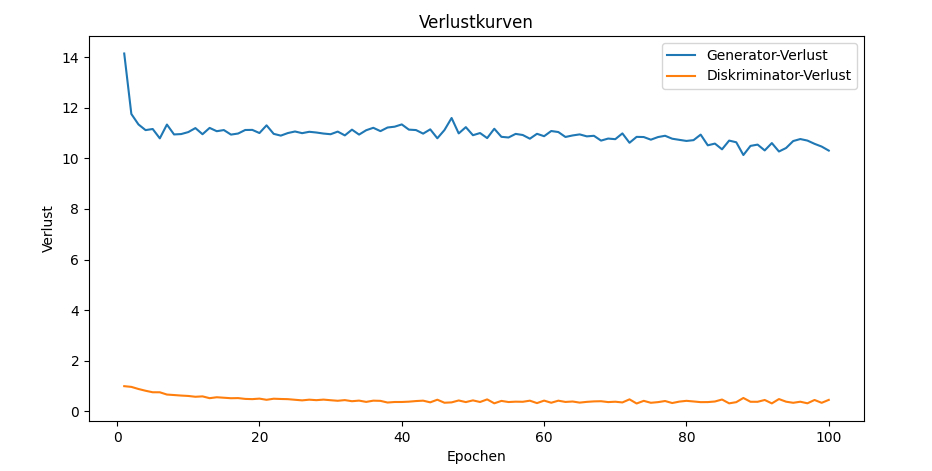
\includegraphics[width=1.0\textwidth]{images/Pix2PixResults/Verlust0-100.png}
	\caption{Generator- und Diskriminatorverlust des 1. Trainingsdurchlaufs mit 100 Epochen, eigene Erstellung mittels matplotlib.pyplot-Bibliothek }
	\label{fig:Verlustkurve 0-100}
\end{figure}

Die Genauigkeit des Diskriminators ist von anfänglich etwa 75$\%$ auf ungefähr 94$\%$ in der letzten Epoche gestiegen. Dies zeigt, dass der Diskriminator im Verlauf des Trainingsprozesses besser darin wurde, echte Bilder von den vom Generator erzeugten Bildern zu unterscheiden.
\begin{figure}[h]
	\centering
	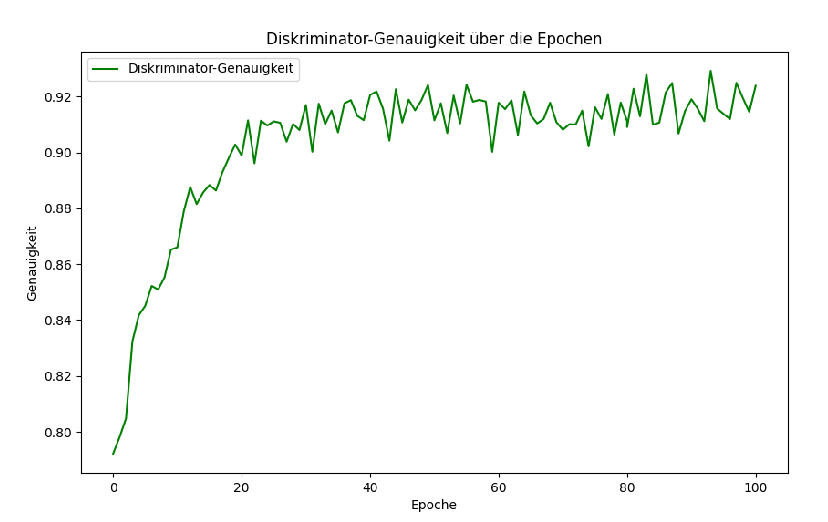
\includegraphics[width=1.0\textwidth]{images/Pix2PixResults/Genauigkeit0-100.png}
	\caption{Diskriminatorgenauigkeit des 1. Trainingsdurchlaufs mit 100 Epochen, eigene Erstellung mittels matplotlib.pyplot-Bibliothek }
	\label{fig:Genauigkeit 0-100}
\end{figure}

Der SSIM-Wert, der die Bildqualität misst, begann bei 0.553 und endete bei 0.656. Diese kontinuierliche Verbesserung deutet darauf hin, dass die generierten Bilder im Laufe des Trainings eine zunehmende Ähnlichkeit mit den Zielbildern erreicht haben.
\begin{figure}[h]
	\centering
	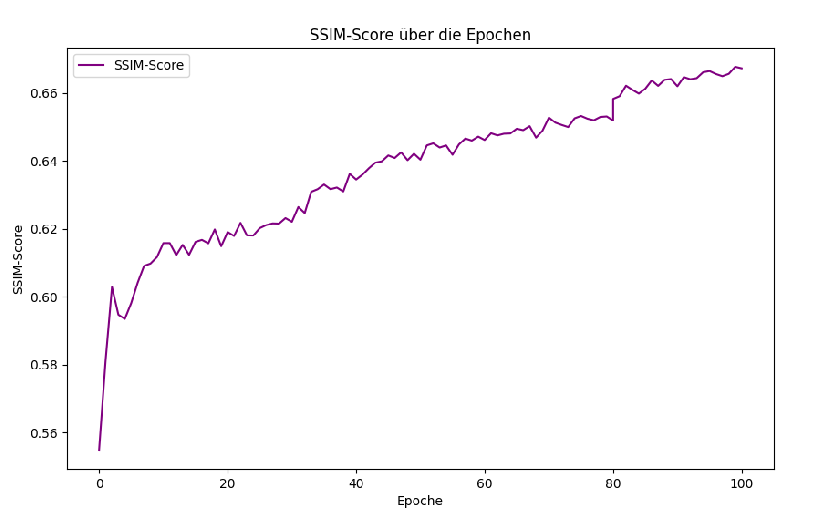
\includegraphics[width=0.95\textwidth]{images/Pix2PixResults/SSIM0-100.png}
	\caption{SSIM-Score des 1. Trainingsdurchlaufs mit 100 Epochen, eigene Erstellung mittels matplotlib.pyplot-Bibliothek}
	\label{fig:SSIM 0-100}
\end{figure}

\newpage
\section{CycleGAN: Ergebnisse und objekte Bewertung}
\section{Vergleich und Bewertung von Pix2Pix und CycleGAN}

\section{Ergebnisse und objektive Bewertung}
In diesem Abschnitt liegt der Fokus auf der objektiven Bewertung der Leistung des CycleGAN-Algorithmus. Es werden verschiedene Metriken und Kriterien herangezogen, um eine umfassende Bewertung durchzuführen, einschließlich der Verluste der Generatoren und Diskriminatoren bei Variation der Hyperparameter. Darüber hinaus wird eine detaillierte Analyse der Genauigkeit der Diskriminatoren und des SSIM-Scores durchgeführt. Diese Messungen sind sowohl für die genaue Bestimmung der Qualität der generierten Ergebnisse als auch für die Bewertung der Lernfähigkeit der Modelle von Bedeutung.

Die verwendeteten Datensätze für die Evaluierung stammen aus dem Berkeley-Repository. Besondere Beachtung wird dem 'maps'-Datensatz geschenkt, bei dem Transformationen zwischen Kartenansichten und Satellitenbildern durchgeführt wurden. Das Training wurde mehrmals mit verschiedenen Hyperparameter-\\Konfigurationen durchgeführt, wobei Parameter wie der Lambda-Wert, die Anzahl der Epochen und die Lernrate des Optimizers variiert wurden. Ziel ist es, eine Konfiguration zu finden, bei der die Qualität der erzeugten Bilder nahe an der Qualität des Originals und die Leistung des Diskriminators optimal ist.

Die subjektive Bewertung erfolgt durch die visuelle Beurteilung der generierten Bilder aus dem Testdatensatz hinsichtlich stimmiger Farben, Struktur und Rauschen im Vergleich zu den Originalbildern. Darauf aufbauend erfolgt eine objektive Bewertung mithilfe der definierten Metriken.


\subsection{Pix2Pix}
 Diese Flexibilität in der Kanalverarbeitung ermöglicht eine breitere Anwendung des Pix2Pix-Modells auf verschiedene Bildtypen. Die Bilder müssen nicht in einer bestimmten Weise vorverarbeitet werden, da das Modell direkt auf den Rohpixeln arbeitet. Diese Flexibilität in der Kanalverarbeitung und die Fähigkeit, direkt auf Rohpixeln zu arbeiten, unterstreichen die Vielseitigkeit des Pix2Pix-Modells.
  Durch empirische Tests hat sich herausgestellt das eine initiale Lernrate von 0.0002 und die Momentum-Parameter von $\beta1$ = 0.5 und $\beta$ = 0.999 optimal sind, um die Balance zwischen Lerngeschwindigkeit und Stabilität des Trainingsprozesses zu optimieren. Auch die Wahl einer kleinen Batchgröße, typischerweise 1, spielt eine entscheidende Rolle, um die Trainingseffizienz zu maximieren und qualitativ hochwertige Ergebnisse zu erzielen. Diese spezifischen Einstellungen der Trainingsparameter tragen maßgeblich dazu bei, das Potenzial des Pix2Pix-Modells voll auszuschöpfen.\cite{PhillipIsola.}.\newline
  Für den Generator und den Diskriminator, wird der Adam-Optimierer mit einer Lernrate von 0.0002 und den Momentum-Parametern $\beta$1 = 0.5 und $\beta$2 = 0.999 verwendet. Diese Einstellungen einen guten Kompromiss zwischen der Lerngeschwindigkeit und der Stabilität des Trainingsprozesses zu finden. Die Batchgröße ist im Code auf 1 gesetzt. Eine kleine Batchgröße kann zu einer höheren Stabilität im Trainingsprozess beitragen. Der Hyperparameter $LAMBDA$ wird verwendet, um das Gewicht des L1-Verlustes im Generatorverlust zu steuern. Ein hoher Wert von $LAMBDA$ betont die Bedeutung der Inhaltsähnlichkeit zwischen den generierten und den Zielbildern. Die Anzahl der Trainingsepochen ist auf 450 gesetzt, was darauf hindeutet, dass das Modell eine umfangreiche Trainingsdauer durchläuft, um eine optimale Leistung zu erreichen.


\subsection{CycleGAN}
Die Datensätze $X$ (Karten) und $Y$ (Satellitenbilder) werden durch die Generatoren $G: X\rightarrow Y$ und $F: Y\rightarrow X$ sowie die Diskriminatoren $D_X$ und $D_Y$ repräsentiert, die jeweils darauf abzielen, Bilder in den Domänen $X$ und $Y$ zu unterscheiden. Die Hyperparameter basieren zunächst auf den in dem Originalpaper von Zhu ausgewählten Parametern und wurden anschließend durch explorative Anpassungen verfeinert.
\\\newline
Ein herausforderndes Problem, dem sich die Generatoren gegenübersehen, besteht in der Reproduktion feiner und detaillierter Strukturen. Insbesondere fällt auf, dass die Generatoren besser darin sind, Straßenlinien zu erzeugen, was auf die Dominanz von Straßen- und Häusermotiven in den Trainingsdaten zurückzuführen ist.
Die Vielfalt in den Bildern, wie Flüsse und Wälder, stellt hingegen eine größere Herausforderung dar. Die Generatoren haben Schwierigkeiten, die Struktur und Farbkodierung dieser Bereiche präzise zu erfassen. Häufig resultiert dies in der Generierung von Flächen mit ähnlicher Farbe wie Straßen, und es werden Versuche unternommen, basierend auf diesen großen Freiflächen kleine Straßen zu generieren.
\\\newline
Die Wahl der Lernrate erwies sich als kritisch, wobei die besten Ergebnisse bei einer Lernrate von $0,0002$ erzielt wurden. Diese Einstellung führte zu den höchsten SSIM-Werten und Diskriminator-Testgenauigkeiten. Insbesondere erzielte der Generator $F$ einen SSIM-Score von $0.592$, während der Generator $G$ einen Wert von $0.198$ erreichte. Die Diskriminatoren zeigten mit $50.1\%$ für $D_Y$ und $48,5\%$ für $D_X$ nahezu optimale Genauigkeiten. Trotz der zunächst hoch erscheinenden visuellen Ähnlichkeit zwischen den generierten Satellitenbildern zeigte eine genauere Analyse, dass kleinere Strukturen im generierten Bild fehlten. Dies spiegelte sich in den vergleichsweise niedrigen SSIM-Wert wider.



\begin{figure}
  \begin{subfigure}[t]{.3\textwidth}
    \centering
    \caption{Input}
    \includegraphics[width=\linewidth]{example-image-a}
  \end{subfigure}
  \hfill
  \begin{subfigure}[t]{.3\textwidth}
    \centering
    \caption{Output}
    \includegraphics[width=\linewidth]{example-image-b}
  \end{subfigure}
  \hfill
  \begin{subfigure}[t]{.3\textwidth}
    \centering
    \caption{Differenzbild}
    \includegraphics[width=\linewidth]{example-image-b}
  \end{subfigure}

  \medskip

  \begin{subfigure}[t]{.3\textwidth}
    \centering
    \includegraphics[width=\linewidth]{example-image-a}
  \end{subfigure}
  \hfill
  \begin{subfigure}[t]{.3\textwidth}
    \centering
    \includegraphics[width=\linewidth]{example-image-b}
  \end{subfigure}
  \hfill
  \begin{subfigure}[t]{.3\textwidth}
    \centering
    \includegraphics[width=\linewidth]{example-image-b}
  \end{subfigure}
  \caption{Testergebnisse nach dem Training mit $\lambda=120$, Lernrate $=0.0002$ und $100$ Epochen}
  \label{evaluation:cycleGan_Testergebnisse}
\end{figure}

\begin{figure}
  \begin{subfigure}[t]{.24\textwidth}
    \centering
    \includegraphics[width=\linewidth]{example-image-a}
    \caption{(a) Generator-Verlust}
  \end{subfigure}
  \begin{subfigure}[t]{.24\textwidth}
    \centering
    \includegraphics[width=\linewidth]{example-image-b}
    \caption{(b) Diskriminator-Metriken}
  \end{subfigure}
  \begin{subfigure}[t]{.24\textwidth}
    \centering
    \includegraphics[width=\linewidth]{example-image-b}
    \caption{(c) SSIM-Score}
  \end{subfigure}
  \begin{subfigure}[t]{.24\textwidth}
    \centering
    \includegraphics[width=\linewidth]{example-image-b}
    \caption{(d) SSIM-Score Zyklus}
  \end{subfigure}

  \caption{Metriken nach dem Training mit $\lambda=120$, Lernrate $=0.0002$ und $100$ Epochen}
  \label{evaluation:cycleGan_Metriken}
\end{figure}


Ebenso zeigten die Bilder bei einem Gewichtungsfaktor von $\lambda = 120$ die besten Resultate, sowohl basierend auf visueller Beurteilung als auch auf dem SSIM-Score (\ref{evaluation:cycleGan_Testergebnisse}). Dieser spezifische Wert für $\lambda$ führte zu generierten Bildern, deren Signal-Rausch-Verhältnis (SNR) entweder besser oder nahezu dem des Originalbildes entspricht. Der SNR-Wert gibt dabei das Verhältnis zwischen dem Signal, repräsentiert durch die relevanten Bildinformationen, und dem Rauschen, repräsentiert durch unerwünschte Störungen, an. In diesem Zusammenhang zeigt ein höherer SNR-Wert eine bessere Qualität und Klarheit der generierten Bilder im Vergleich zu Rauschen.
\\\newline
Trotz dieser Erfolge bleibt das Training instabil, und es besteht die Möglichkeit eines Modekollapses. Die Generatoren zeigen Anzeichen eines exponentiellen Verfalls in ihren Verlustkurven, während der SSIM-Score nur langsam ansteigt. Dies deutet darauf hin, dass die Generatoren zwar ihre Verluste minimieren, jedoch möglicherweise nicht die gewünschte visuelle Qualität erreichen (\ref{evaluation:cycleGan_Metriken}).

\begin{figure}
  \begin{subfigure}[t]{.2\textwidth}
    \caption{Input}
    \centering
    \includegraphics[width=\linewidth]{example-image-a}
  \end{subfigure}
  \begin{subfigure}[t]{.2\textwidth}
    \caption{Output}
    \centering
    \includegraphics[width=\linewidth]{example-image-b}
  \end{subfigure}
  \hfill
  \begin{subfigure}[t]{.2\textwidth}
    \caption{Input}
    \centering
    \includegraphics[width=\linewidth]{example-image-a}
  \end{subfigure}
  \begin{subfigure}[t]{.2\textwidth}
    \caption{Output}
    \centering
    \includegraphics[width=\linewidth]{example-image-b}
  \end{subfigure}

  \medskip

  \begin{subfigure}[t]{.2\textwidth}
    \centering
    \includegraphics[width=\linewidth]{example-image-a}
  \end{subfigure}
  \begin{subfigure}[t]{.2\textwidth}
    \centering
    \includegraphics[width=\linewidth]{example-image-b}
  \end{subfigure}
  \hfill
  \begin{subfigure}[t]{.2\textwidth}
    \centering
    \includegraphics[width=\linewidth]{example-image-a}
  \end{subfigure}
  \begin{subfigure}[t]{.2\textwidth}
    \centering
    \includegraphics[width=\linewidth]{example-image-b}
  \end{subfigure}

  \medskip

  \begin{subfigure}[t]{.2\textwidth}
    \centering
    \includegraphics[width=\linewidth]{example-image-a}
  \end{subfigure}
  \begin{subfigure}[t]{.2\textwidth}
    \centering
    \includegraphics[width=\linewidth]{example-image-b}
  \end{subfigure}
  \hfill
  \begin{subfigure}[t]{.2\textwidth}
    \centering
    \includegraphics[width=\linewidth]{example-image-a}
  \end{subfigure}
  \begin{subfigure}[t]{.2\textwidth}
    \centering
    \includegraphics[width=\linewidth]{example-image-b}
  \end{subfigure}

  \medskip

  \begin{subfigure}[t]{.2\textwidth}
    \centering
    \includegraphics[width=\linewidth]{example-image-a}
  \end{subfigure}
  \begin{subfigure}[t]{.2\textwidth}
    \centering
    \includegraphics[width=\linewidth]{example-image-b}
  \end{subfigure}
  \hfill
  \begin{subfigure}[t]{.2\textwidth}
    \centering
    \includegraphics[width=\linewidth]{example-image-a}
  \end{subfigure}
  \begin{subfigure}[t]{.2\textwidth}
    \centering
    \includegraphics[width=\linewidth]{example-image-b}
  \end{subfigure}
  \caption{Beste Ergebnisse des Trainings}

\end{figure}


Die generierten Bilder weisen bereits zu diesem Zeitpunkt eine grobe visuelle Ähnlichkeit mit der Struktur des zugrunde liegenden Originalbildes auf und zeigen nur minimale Variationen. Allerdings wird durch den SSIM-Score deutlich, dass die Generatoren Schwierigkeiten haben, bedeutende Verbesserungen hinsichtlich feinerer Details und Farbübereinstimmungen zu erzielen. Diese lassen sich auch visuell in den Differenzbilder, die mit Hilfe eines Histogrammsausgleich kontrastverstärkt wurden, erkennen. Helle Bereiche in diesen Differenzbildern stellen dabei größere Unterschiede dar. Dabei sammeln sich helle Bereiche vor allem bei den kleinen pixelweisen Details an, sowie bei unterschiedlichen Farbkodierungen. Ein konkretes Beispiel ist in Abbildung \ref{evaluation:cycleGan_Testergebnisse} zu sehen.
\\
Insbesondere in den frühen Epochen sind die Generatoren nicht in der Lage, Straßenlinien zuverlässig als gerade Linien zu generieren. Diese Schwächen verbessern sich im Laufe längerer Trainingszeiten, wobei bereits nach etwa 300 Epochen relativ konsistente, gerade Linien erzeugt werden.
\\\newline
Die Analyse des SSIM-Scores im Kontext der Zyklusübersetzung offenbart eine exponentielle Zunahme. Diese Beobachtung legt nahe, dass der Zykluskonsistenz-Verlust einen erheblichen Einfluss auf das Training ausübt. Die exponentielle Steigerung des SSIM-Scores deutet darauf hin, dass die Konsistenz zwischen den Original- und zurückübersetzten Bildern im Laufe der Zeit kontinuierlich zunimmt. Dies könnte auf eine fortlaufende Verbesserung der Generatoren hinsichtlich ihrer Fähigkeit zur Zyklusübersetzung hindeuten. Insgesamt erreichen die SSIM-Scores für die Zyklusübersetzung Werte von $80\%$ für $Y$ und $90\%$ für $X$ (\ref{evaluation:cycleGan_Metriken}).

\begin{table}
\centering
\begin{tabular}{|l|l|l|l|l|l|l|l|l|l|l|l|l|l|l|}
\hline
\textbf{Lambda} &
  \textbf{Epoche} &
  \textbf{Lernrate} &
  \textbf{\begin{tabular}[c]{@{}l@{}}$D_Y$ \\ Tr-Acc\end{tabular}} &
  \textbf{\begin{tabular}[c]{@{}l@{}}$D_X$ \\ Tr-Acc\end{tabular}} &
  \textbf{\begin{tabular}[c]{@{}l@{}}$D_Y$ \\ Te-Acc\end{tabular}} &
  \textbf{\begin{tabular}[c]{@{}l@{}}$D_X$ \\ Te-Acc\end{tabular}} \\ \hline
120 & 100 & 0.000025 & 0.549 & 0.494 & 0.307 & 0.497   \\ \hline
120 & 100 & 0.00005  & 0.537 & 0.491 & 0.321 & 0.489 \\ \hline
120 & 100 & 0.0001   & 0.519 & 0.490 & 0.418 & 0.485 \\ \hline
120 & 100 & 0.0002   & 0.518 & 0.495 & 0.501 & 0.485 \\ \hline
120 & 100 & 0.0004   & 0.516 & 0.487 & 0.462 & 0.496 \\ \hline
100 & 100 & 0.0002   & 0.521 & 0.491 & 0.527 & 0.481   \\ \hline
140 & 100 & 0.0002   & 0.562 & 0.492 & 0.544 & 0.469 \\ \hline
100 & 300 & 0.0002   & 0.51  & 0.484 & 0.47  & 0.676 \\ \hline
120 & 300 & 0.0002   & 0.508 & 0.495 & 0.468 & 0.709  \\ \hline
\end{tabular}
\caption{CycleGAN Ergebnisse unter verschiedenen Hyperparameter Teil1}
\label{evaluation:cycleGan_table1}
\end{table}

\begin{table}
\centering
\begin{tabular}{|l|l|l|l|l|l|l|l|l|l|l|l|l|l|l|}
\hline
\textbf{\begin{tabular}[c]{@{}l@{}}$F$\\ Loss\end{tabular}} &
\textbf{\begin{tabular}[c]{@{}l@{}}$G$\\ Loss\end{tabular}} &
  \textbf{\begin{tabular}[c]{@{}l@{}}$X$ \\ SSIM\end{tabular}} &
  \textbf{\begin{tabular}[c]{@{}l@{}}$Y$ \\SSIM \end{tabular}} &
  \textbf{\begin{tabular}[c]{@{}l@{}}$X$\\Z-SSIM\end{tabular}} &
  \textbf{\begin{tabular}[c]{@{}l@{}}$Y$ \\ Z-SSIM\end{tabular}} &
  \textbf{\begin{tabular}[c]{@{}l@{}}$X$\\SNR \end{tabular}} &
  \textbf{\begin{tabular}[c]{@{}l@{}}$Y$\\SNR\end{tabular}} \\ \hline
53.113 & 22.556 & 0.545 & 0.191 & 0.895 & 0.831 & -2.991 & 0.228  \\ \hline
44.626 & 20.417 & 0.541 & 0.191 & 0.916 & 0.836 & -0.589 & 1.071  \\ \hline
44.376 & 21.943 & 0.580 & 0.194 & 0.935 & 0.842 & -4.604 & 1.367  \\ \hline
42.489 & 22.373 & 0.592 & 0.198 & 0.921 & 0.796 & -5.308 & 0.851  \\ \hline
46.972 & 28.175 & 0.585 & 0.209 & 0.856 & 0.602 &        &        \\ \hline
34.973 & 18.837 & 0.551 & 0.194 & 0.93  & 0.83  & -3.292 & 1.261  \\ \hline
13.048 & 6.842  & 0.510 & 0.179 & 0.513 & 0.409 & -2.087 & 1.005  \\ \hline
34.881 & 20.899 & 0.577 & 0.191 & 0.931 & 0.756 & -2.705 & 1.373  \\ \hline
46.652 & 26.360 & 0.585 & 0.207 & 0.901 & 0.707 & 1.248  & -3.409 \\ \hline
\end{tabular}
\caption{CycleGAN Ergebnisse unter verschiedenen Hyperparameter Teil2}
\label{evaluation:cycleGan_table2}
\end{table}


Im Kontrast dazu bleibt die Genauigkeit der Diskriminatoren für Trainingsdaten stabil bei etwa $50\%$. Jedoch zeigen sich erhebliche Schwankungen je nach Epoche für die Testdaten, insbesondere für $D_Y$. Dies legt nahe, dass die Diskriminatoren möglicherweise Schwierigkeiten haben, mit neuen, nicht trainierten Daten umzugehen. Diese Schwankungen könnten auf Überanpassung oder eine mangelnde Generalisierungsfähigkeit des Modells hinweisen, trotz der implementierten Maßnahmen wie dem Hinzufügen von Rauschen und Dropout-Schichten (\ref{evaluation:cycleGan_Metriken}).
\\\newline
Die Laufzeit des Trainings spiegelt die Komplexität der Modelle wider, insbesondere auf der GPU, wo jede Epoche im Durchschnitt etwa 2 Minuten dauert. Im Vergleich dazu benötigt die CPU, selbst nach einer Reduzierung der Residualblöcke auf einen Block, rund 6 Minuten pro Epoche. Die Nutzung von Instanznormalisierung trägt zur beschleunigten Konvergenz und Verbesserung der Laufzeit bei. Zudem zeigt sich, dass die Verwendung von Residualblöcken eine bessere Laufzeit ermöglicht im Vergleich zu Generatoren mit zusätzlichen Schichten. 
\\\newline
Insgesamt zeigt die Evaluation, dass das CycleGAN-Modell trotz einiger Herausforderungen in der Generierung von detaillierten Strukturen und der Generalisierung auf neue Daten vielversprechende Ergebnisse erzielt.


\section{Vergleich von Pix2Pix und CycleGAN}
- Matching Paare von Bildern sind ebenfalls für das Training nicht nötig (crewall)
- Macht die Datenvorbereitung einfacher und öffnet neue Techniken für Applikationen (crewall)